\subsection{MNIST Data Set and Feature Selection}

We applied a perceptron model to classification of handwritten digits. MNIST is a standard data set with $28\times28$ pixel images of handwritten digits.
We selected the digits $0$ and $7$ and 500 training images for each class for our classification task, as they are reasonably diffenrent. To chose the right feature we plotted all regionprops in a scatter plot matrix,see figure \ref{perceptron:features} and selected solodity and eccentricity.

\begin{figure}
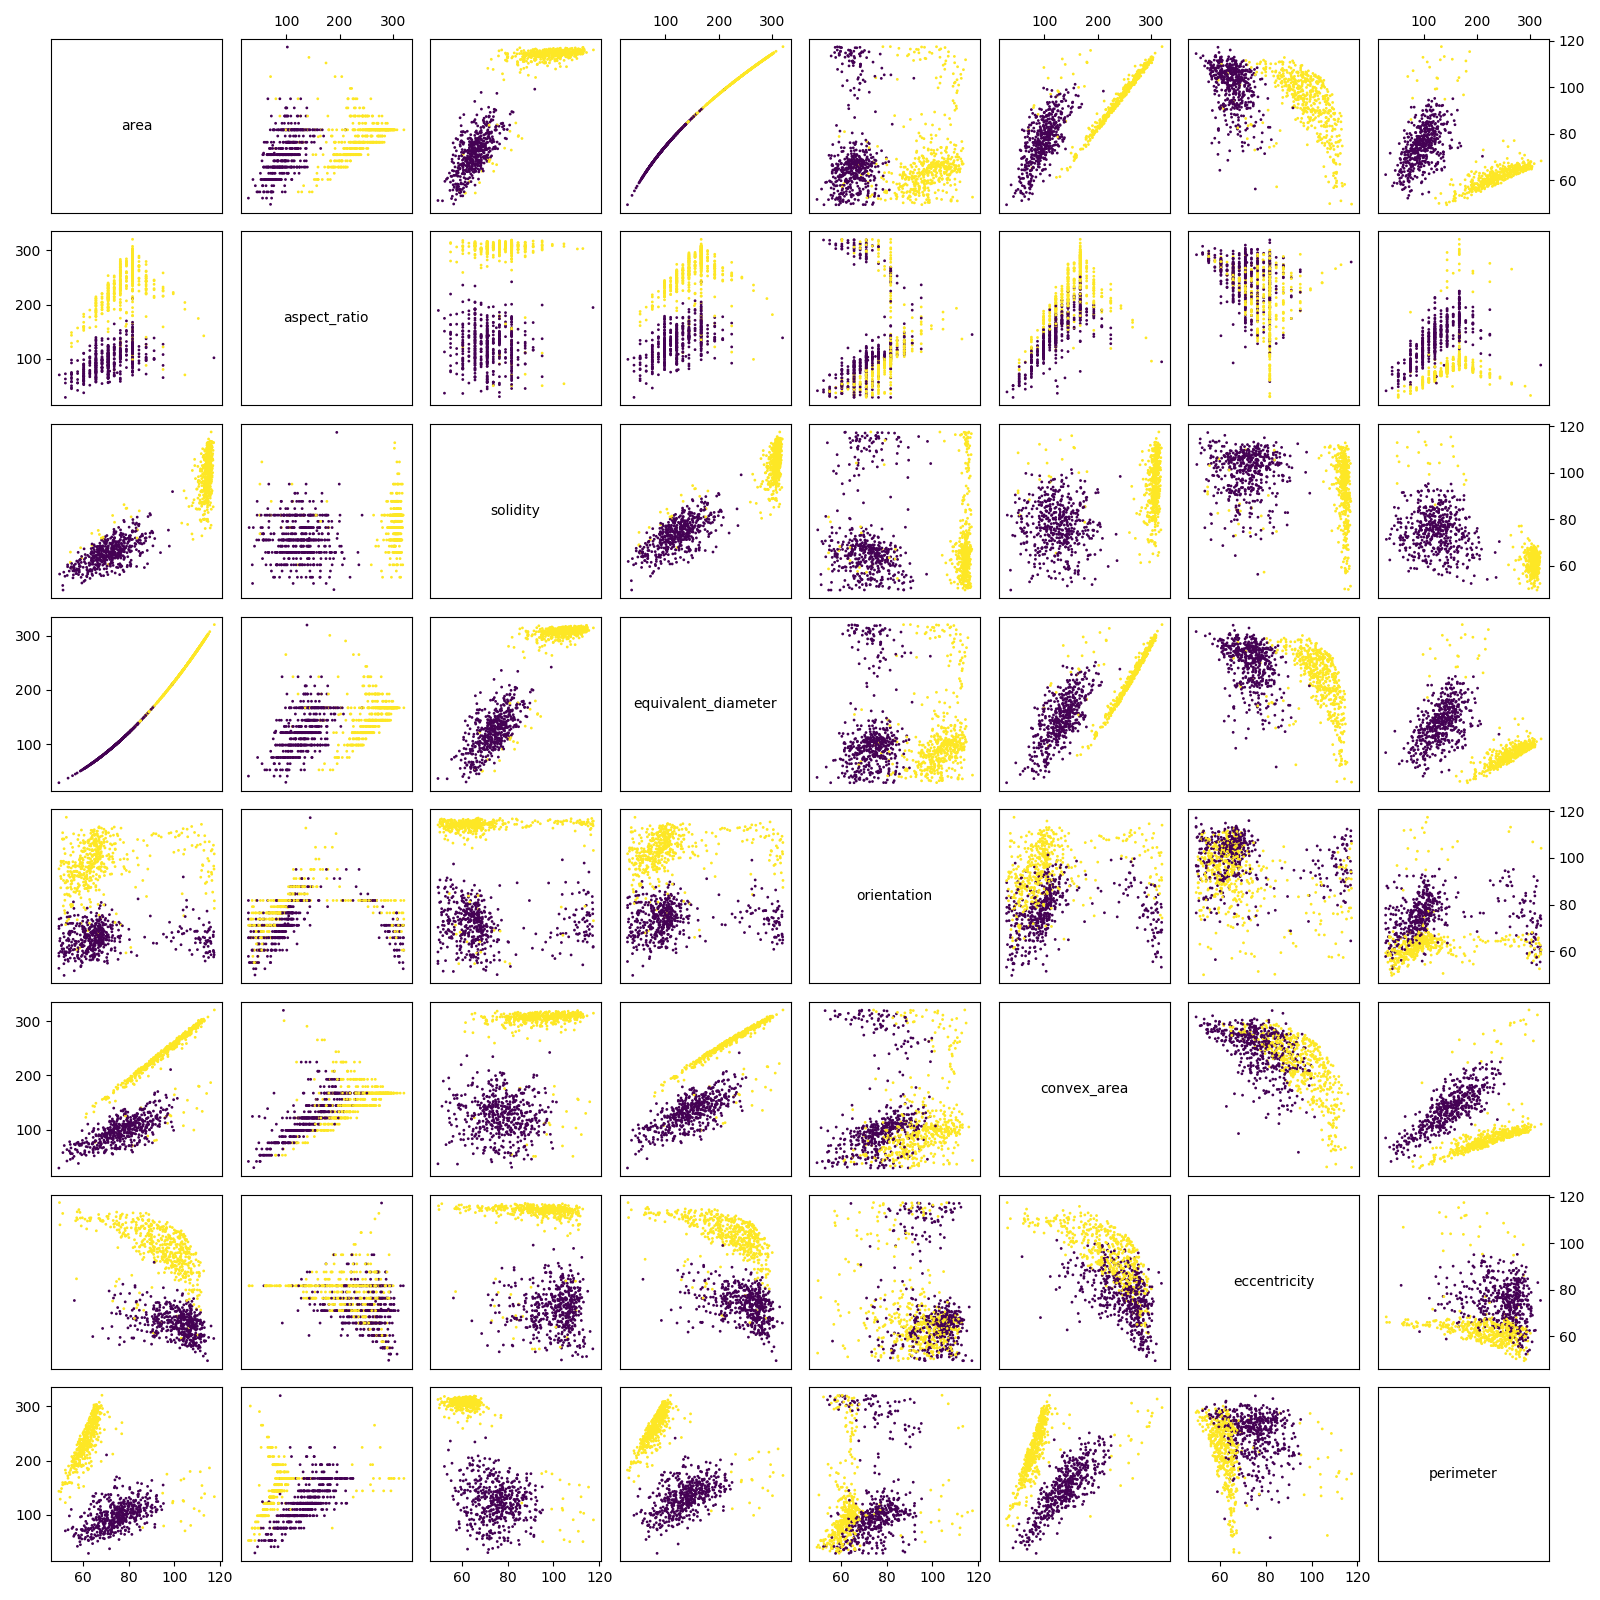
\includegraphics{figures/scatter_matrix}
\caption{Scatter plot matrix of all region properties}
\label{perceptron:features}
\end{figure}

\subsubsection{Features without transform}

We used once the batch training algorithm and once the online training algorithm to classify the data directly from these to features. The connfusion matrix evaluated on a separate test set gives us following perfomance:

Tabelle1

Tabelle2

The corresponding decision boundries are shown in figure ... . We see that the data is not linearly seperable

\subsubsection{Classification with feature transform}

\subsubsection{Classification directly with image data}
